\subsection{IASI Band 1 (645-1210\invcm)}
%----------------------------------------

\subsubsection{WVO results}
%..........................
IASI band 1 brightness temperature residuals for all the WVO1 set of transmittances are shown in figure \ref{fig:iasiB1.wvo1_dtb_sfc}, with the average, RMS, and maximum residuals shown in figure \ref{fig:iasiB1.wvo1_dtb}. Figures \ref{fig:iasiB1.wvo2_dtb_sfc} and \ref{fig:iasiB1.wvo2_dtb} show the same for the WVO2 set of transmittances.

The largest residuals for the WVO set of transmittances are concentrated in the shortwave portion of the \carbondioxide{} 15\micron{} band edge from $\sim$700-800\invcm, in the 9.6\micron{} \ozone{} region (980-1080\invcm), and the 8\micron{} midwave window region (1100-1200\invcm). The WVO2 results appear better behaved in general, with a much smaller RMS residual and fewer large residuals throught the band.
\begin{figure}[htp]
  \centering
  \includegraphics[scale=0.8]{graphics/iasiB1/iasiB1.wvo1_dtb_sfc.eps}
  \caption{IASI band 1 brightness temperature residuals for all view angles and profiles between using the true total transmittance profiles and those derived from the WVO1 set (see table \ref{tab:derived_set_combo})}
  \label{fig:iasiB1.wvo1_dtb_sfc}
  \vspace{1em}
  \includegraphics[scale=0.8]{graphics/iasiB1/iasiB1.wvo1_dtb.eps}
  \caption{IASI band 1 brightness temperature residual statistics between using the true total transmittance profiles and those derived from the WVO1 set (see table \ref{tab:derived_set_combo}). Compiled for all view angle and profile combinations. \textbf{(Top panel)} Average T\subscript{B} residuals. \textbf{(Middle panel)} RMS T\subscript{B} residuals. \textbf{(Bottom panel)} Maximum T\subscript{B} residuals.}
  \label{fig:iasiB1.wvo1_dtb}
\end{figure}
\begin{figure}[htp]
  \centering
  \includegraphics[scale=0.8]{graphics/iasiB1/iasiB1.wvo2_dtb_sfc.eps}
  \caption{IASI band 1 brightness temperature residuals for all view angles and profiles between using the true total transmittance profiles and those derived from the WVO2 set (see table \ref{tab:derived_set_combo})}
  \label{fig:iasiB1.wvo2_dtb_sfc}
  \vspace{1em}
  \includegraphics[scale=0.8]{graphics/iasiB1/iasiB1.wvo2_dtb.eps}
  \caption{IASI band 1 brightness temperature residual statistics between using the true total transmittance profiles and those derived from the WVO2 set (see table \ref{tab:derived_set_combo}). Compiled for all view angle and profile combinations. \textbf{(Top panel)} Average T\subscript{B} residuals. \textbf{(Middle panel)} RMS T\subscript{B} residuals. \textbf{(Bottom panel)} Maximum T\subscript{B} residuals.}
  \label{fig:iasiB1.wvo2_dtb}
\end{figure}


\subsubsection{DOZ results}
%..........................
IASI band 1 brightness temperature residuals for all the DOZ1 set of transmittances are shown in figure \ref{fig:iasiB1.doz1_dtb_sfc}, with the average, RMS, and maximum residuals shown in figure \ref{fig:iasiB1.doz1_dtb}. Figures \ref{fig:iasiB1.doz2_dtb_sfc} and \ref{fig:iasiB1.doz2_dtb} show the same for the DOZ2 set of transmittances.

The largest residuals for the DOZ set of transmittances occur in the DOZ1 set with a cluster of large residuals in the \carbondioxide{} 15\micron{} band up to $\sim$770\invcm (see figure \ref{fig:iasiB1.doz1_dtb}). The residuals for the DOZ2 transmittance set are much better behaved to the extent that the residuals are mostly dominated by the ringing due to the instrument apodisation (see figure \ref{fig:iasiB1.doz2_dtb}).
\begin{figure}[htp]
  \centering
  \includegraphics[scale=0.8]{graphics/iasiB1/iasiB1.doz1_dtb_sfc.eps}
  \caption{IASI band 1 brightness temperature residuals for all view angles and profiles between using the true total transmittance profiles and those derived from the DOZ1 set (see table \ref{tab:derived_set_combo})}
  \label{fig:iasiB1.doz1_dtb_sfc}
  \vspace{1em}
  \includegraphics[scale=0.8]{graphics/iasiB1/iasiB1.doz1_dtb.eps}
  \caption{IASI band 1 brightness temperature residual statistics between using the true total transmittance profiles and those derived from the DOZ1 set (see table \ref{tab:derived_set_combo}). Compiled for all view angle and profile combinations. \textbf{(Top panel)} Average T\subscript{B} residuals. \textbf{(Middle panel)} RMS T\subscript{B} residuals. \textbf{(Bottom panel)} Maximum T\subscript{B} residuals.}
  \label{fig:iasiB1.doz1_dtb}
\end{figure}
\begin{figure}[htp]
  \centering
  \includegraphics[scale=0.8]{graphics/iasiB1/iasiB1.doz2_dtb_sfc.eps}
  \caption{IASI band 1 brightness temperature residuals for all view angles and profiles between using the true total transmittance profiles and those derived from the DOZ2 set (see table \ref{tab:derived_set_combo})}
  \label{fig:iasiB1.doz2_dtb_sfc}
  \vspace{1em}
  \includegraphics[scale=0.8]{graphics/iasiB1/iasiB1.doz2_dtb.eps}
  \caption{IASI band 1 brightness temperature residual statistics between using the true total transmittance profiles and those derived from the DOZ2 set (see table \ref{tab:derived_set_combo}). Compiled for all view angle and profile combinations. \textbf{(Top panel)} Average T\subscript{B} residuals. \textbf{(Middle panel)} RMS T\subscript{B} residuals. \textbf{(Bottom panel)} Maximum T\subscript{B} residuals.}
  \label{fig:iasiB1.doz2_dtb}
\end{figure}


\subsubsection{WVD results}
%..........................
IASI band 1 brightness temperature residuals for all the WVD1 set of transmittances are shown in figure \ref{fig:iasiB1.wvd1_dtb_sfc}, with the average, RMS, and maximum residuals shown in figure \ref{fig:iasiB1.wvd1_dtb}. Figures \ref{fig:iasiB1.wvd2_dtb_sfc} and \ref{fig:iasiB1.wvd2_dtb} show the same for the WVD2 set of transmittances.

Both sets of WVD residuals appear to combine the worst effects of the WVO and DOZ results. Comparison of the WVD surface plots indicate the WVD2 residuals are smaller at the shortwave end of the band for some angle/profile combinations, but overall the statistics for each set are very similar.
\begin{figure}[htp]
  \centering
  \includegraphics[scale=0.8]{graphics/iasiB1/iasiB1.wvd1_dtb_sfc.eps}
  \caption{IASI band 1 brightness temperature residuals for all view angles and profiles between using the true total transmittance profiles and those derived from the WVD1 set (see table \ref{tab:derived_set_combo})}
  \label{fig:iasiB1.wvd1_dtb_sfc}
  \vspace{1em}
  \includegraphics[scale=0.8]{graphics/iasiB1/iasiB1.wvd1_dtb.eps}
  \caption{IASI band 1 brightness temperature residual statistics between using the true total transmittance profiles and those derived from the WVD1 set (see table \ref{tab:derived_set_combo}). Compiled for all view angle and profile combinations. \textbf{(Top panel)} Average T\subscript{B} residuals. \textbf{(Middle panel)} RMS T\subscript{B} residuals. \textbf{(Bottom panel)} Maximum T\subscript{B} residuals.}
  \label{fig:iasiB1.wvd1_dtb}
\end{figure}
\begin{figure}[htp]
  \centering
  \includegraphics[scale=0.8]{graphics/iasiB1/iasiB1.wvd2_dtb_sfc.eps}
  \caption{IASI band 1 brightness temperature residuals for all view angles and profiles between using the true total transmittance profiles and those derived from the WVD2 set (see table \ref{tab:derived_set_combo})}
  \label{fig:iasiB1.wvd2_dtb_sfc}
  \vspace{1em}
  \includegraphics[scale=0.8]{graphics/iasiB1/iasiB1.wvd2_dtb.eps}
  \caption{IASI band 1 brightness temperature residual statistics between using the true total transmittance profiles and those derived from the WVD2 set (see table \ref{tab:derived_set_combo}). Compiled for all view angle and profile combinations. \textbf{(Top panel)} Average T\subscript{B} residuals. \textbf{(Middle panel)} RMS T\subscript{B} residuals. \textbf{(Bottom panel)} Maximum T\subscript{B} residuals.}
  \label{fig:iasiB1.wvd2_dtb}
\end{figure}
